\documentclass[11pt,a4paper]{article}

\usepackage[toc,page]{appendix}
\usepackage{amsmath, amssymb}
\usepackage{bm}% bold math
\usepackage{cancel, caption}
\usepackage{dcolumn}% Align table columns on decimal point
\usepackage{epsfig, epsf}
\usepackage{graphicx,fancyhdr,natbib,subfigure}
\usepackage{lscape, longtable}
\usepackage{hyperref,ifthen}
\usepackage{verbatim}
\usepackage{color}
\usepackage[usenames,dvipsnames]{xcolor}
\usepackage{listings}
%% http://en.wikibooks.org/wiki/LaTeX/Colors



%%%%%%%%%%%%%%%%%%%%%%%%%%%%%%%%%%%%%%%%%%%
%       define Journal abbreviations      %
%%%%%%%%%%%%%%%%%%%%%%%%%%%%%%%%%%%%%%%%%%%
\def\nat{Nat} \def\apjl{ApJ~Lett.} \def\apj{ApJ}
\def\apjs{ApJS} \def\aj{AJ} \def\mnras{MNRAS}
\def\prd{Phys.~Rev.~D} \def\prl{Phys.~Rev.~Lett.}
\def\plb{Phys.~Lett.~B} \def\jhep{JHEP} \def\nar{NewAR}
\def\npbps{NUC.~Phys.~B~Proc.~Suppl.} \def\prep{Phys.~Rep.}
\def\pasp{PASP} \def\aap{Astron.~\&~Astrophys.} \def\araa{ARA\&A}
\def\jcap{\ref@jnl{J. Cosmology Astropart. Phys.}}%
\def\physrep{Phys.~Rep.}

\newcommand{\preep}[1]{{\tt #1} }

%%%%%%%%%%%%%%%%%%%%%%%%%%%%%%%%%%%%%%%%%%%%%%%%%%%%%
%              define symbols                       %
%%%%%%%%%%%%%%%%%%%%%%%%%%%%%%%%%%%%%%%%%%%%%%%%%%%%%
\def \Mpc {~{\rm Mpc} }
\def \Om {\Omega_0}
\def \Omb {\Omega_{\rm b}}
\def \Omcdm {\Omega_{\rm CDM}}
\def \Omlam {\Omega_{\Lambda}}
\def \Omm {\Omega_{\rm m}}
\def \ho {H_0}
\def \qo {q_0}
\def \lo {\lambda_0}
\def \kms {{\rm ~km~s}^{-1}}
\def \kmsmpc {{\rm ~km~s}^{-1}~{\rm Mpc}^{-1}}
\def \hmpc{~\;h^{-1}~{\rm Mpc}} 
\def \hkpc{\;h^{-1}{\rm kpc}} 
\def \hmpcb{h^{-1}{\rm Mpc}}
\def \dif {{\rm d}}
\def \mlim {m_{\rm l}}
\def \bj {b_{\rm J}}
\def \mb {M_{\rm b_{\rm J}}}
\def \mg {M_{\rm g}}
\def \qso {_{\rm QSO}}
\def \lrg {_{\rm LRG}}
\def \gal {_{\rm gal}}
\def \xibar {\bar{\xi}}
\def \xis{\xi(s)}
\def \xisp{\xi(\sigma, \pi)}
\def \Xisig{\Xi(\sigma)}
\def \xir{\xi(r)}
\def \max {_{\rm max}}
\def \gsim { \lower .75ex \hbox{$\sim$} \llap{\raise .27ex \hbox{$>$}} }
\def \lsim { \lower .75ex \hbox{$\sim$} \llap{\raise .27ex \hbox{$<$}} }
\def \deg {^{\circ}}
%\def \sqdeg {\rm deg^{-2}}
\def \deltac {\delta_{\rm c}}
\def \mmin {M_{\rm min}}
\def \mbh  {M_{\rm BH}}
\def \mdh  {M_{\rm DH}}
\def \msun {M_{\odot}}
\def \z {_{\rm z}}
\def \edd {_{\rm Edd}}
\def \lin {_{\rm lin}}
\def \nonlin {_{\rm non-lin}}
\def \wrms {\langle w_{\rm z}^2\rangle^{1/2}}
\def \dc {\delta_{\rm c}}
\def \wp {w_{p}(\sigma)}
\def \PwrSp {\mathcal{P}(k)}
\def \DelSq {$\Delta^{2}(k)$}
\def \WMAP {{\it WMAP \,}}
\def \cobe {{\it COBE }}
\def \COBE {{\it COBE \;}}
\def \HST  {{\it HST \,\,}}
\def \Spitzer  {{\it Spitzer \,}}
\def \ATLAS {VST-AA$\Omega$ {\it ATLAS} }
\def \BEST   {{\tt best} }
\def \TARGET {{\tt target} }
\def \TQSO   {{\tt TARGET\_QSO}}
\def \HIZ    {{\tt TARGET\_HIZ}}
\def \FIRST  {{\tt TARGET\_FIRST}}
\def \zc {z_{\rm c}}
\def \zcz {z_{\rm c,0}}

\newcommand{\ltsim}{\raisebox{-0.6ex}{$\,\stackrel
        {\raisebox{-.2ex}{$\textstyle <$}}{\sim}\,$}}
\newcommand{\gtsim}{\raisebox{-0.6ex}{$\,\stackrel
        {\raisebox{-.2ex}{$\textstyle >$}}{\sim}\,$}}
\newcommand{\simlt}{\raisebox{-0.6ex}{$\,\stackrel
        {\raisebox{-.2ex}{$\textstyle <$}}{\sim}\,$}}
\newcommand{\simgt}{\raisebox{-0.6ex}{$\,\stackrel
        {\raisebox{-.2ex}{$\textstyle >$}}{\sim}\,$}}

\newcommand{\Msun}{M_\odot}
\newcommand{\Lsun}{L_\odot}
\newcommand{\lsun}{L_\odot}
\newcommand{\Mdot}{\dot M}

\newcommand{\sqdeg}{deg$^{-2}$}
\newcommand{\lya}{Ly$\alpha$\ }
%\newcommand{\lya}{Ly\,$\alpha$\ }
\newcommand{\lyaf}{Ly\,$\alpha$\ forest}
%\newcommand{\eg}{e.g.~}
%\newcommand{\etal}{et~al.~}
\newcommand{\lyb}{Ly$\beta$\ }
\newcommand{\cii}{C\,{\sc ii}\ }
\newcommand{\ciii}{C\,{\sc iii}]\ }
\newcommand{\civ}{C\,{\sc iv}\ }
\newcommand{\SiIV}{Si\,{\sc iv}\ }
\newcommand{\mgii}{Mg\,{\sc ii}\ }
\newcommand{\feii}{Fe\,{\sc ii}\ }
\newcommand{\feiii}{Fe\,{\sc iii}\ }
\newcommand{\caii}{Ca\,{\sc ii}\ }
\newcommand{\halpha}{H\,$\alpha$\ }
\newcommand{\hbeta}{H\,$\beta$\ }
\newcommand{\hgamma}{H\,$\gamma$\ }
\newcommand{\hdelta}{H\,$\delta$\ }
\newcommand{\oi}{[O\,{\sc i}]\ }
\newcommand{\oii}{[O\,{\sc ii}]\ }
\newcommand{\oiii}{[O\,{\sc iii}]\ }
\newcommand{\heii}{[He\,{\sc ii}]\ }
\newcommand{\nv}{N\,{\sc v}\ }
\newcommand{\nev}{Ne\,{\sc v}\ }
\newcommand{\neiii}{[Ne\,{\sc iii}]\ }
\newcommand{\aliii}{Al\,{\sc iii}\ }
\newcommand{\siiii}{Si\,{\sc iii}]\ }


%%%%%%%%%%%%%%%%%%%%%%%%%%%%%%%%%%%%%%%%%%%%%%%%%%%%%
%              define Listings                       %
%%%%%%%%%%%%%%%%%%%%%%%%%%%%%%%%%%%%%%%%%%%%%%%%%%%%%
\definecolor{dkgreen}{rgb}{0,0.6,0}
\definecolor{gray}{rgb}{0.5,0.5,0.5}
\definecolor{mauve}{rgb}{0.58,0,0.82}

\lstset{frame=tb,
  language=Python,
  aboveskip=3mm,
  belowskip=3mm,
  showstringspaces=false,
  columns=flexible,
  basicstyle={\small\ttfamily},
  numbers=none,
  numberstyle=\tiny\color{gray},
  keywordstyle=\color{blue},
  commentstyle=\color{dkgreen},
  stringstyle=\color{mauve},
  breaklines=true,
  breakatwhitespace=true,
  tabsize=3
}

\begin{document}

   \title{Topic Model Equations}
  \author{npr}
 \date{\today}
\maketitle


The normalizing constant is the multivariate Beta function, which can be expressed in terms of the gamma function:

\begin{equation}
\mathrm {B} ({\boldsymbol {\alpha }})={\frac {\prod _{i=1}^{K}\Gamma (\alpha _{i})}{\Gamma \left(\sum _{i=1}^{K}\alpha _{i}\right)}},\qquad {\boldsymbol {\alpha }}=(\alpha _{1},\cdots ,\alpha _{K}).
\end{equation}
where $K\geq 2$ number of categories (integer) and \\
$\alpha_{1},\cdots ,\alpha_{K}$ concentration parameters, where $\alpha_{i}>0 \alpha_{i}>0$.

\begin{equation}
P(\mathbf{p}| \alpha m) =  \frac{\Gamma(\sum_{k}\; \alpha \, m_k) }{\prod_{k}\Gamma(\alpha \, m_k)}\prod_{k} \, p_{k}^{\alpha m_k -1}
\end{equation}

\smallskip
\smallskip
\noindent
e.g. Slide at 13:02 in the \href{https://www.youtube.com/watch?v=yK7nN3FcgUs&t=715s}{\tt Topic Models} Youtube video:
\begin{eqnarray}
p(\phi | \alpha, {\bf w})  & \propto & p({\bf w} | \phi) \;  p(\phi|\alpha) \\
                                       & \propto & \prod_{k} \phi^{n_{k}}  \; \prod_{k} \phi^{\alpha_{k}-1}\\ 
                                       & \propto & \prod_{k} \phi^{n_{k} + \alpha_{k}-1}
\end{eqnarray}
$K$ topics\\





\subsection{LDA Plate Notation}
\begin{figure}
	\centering
	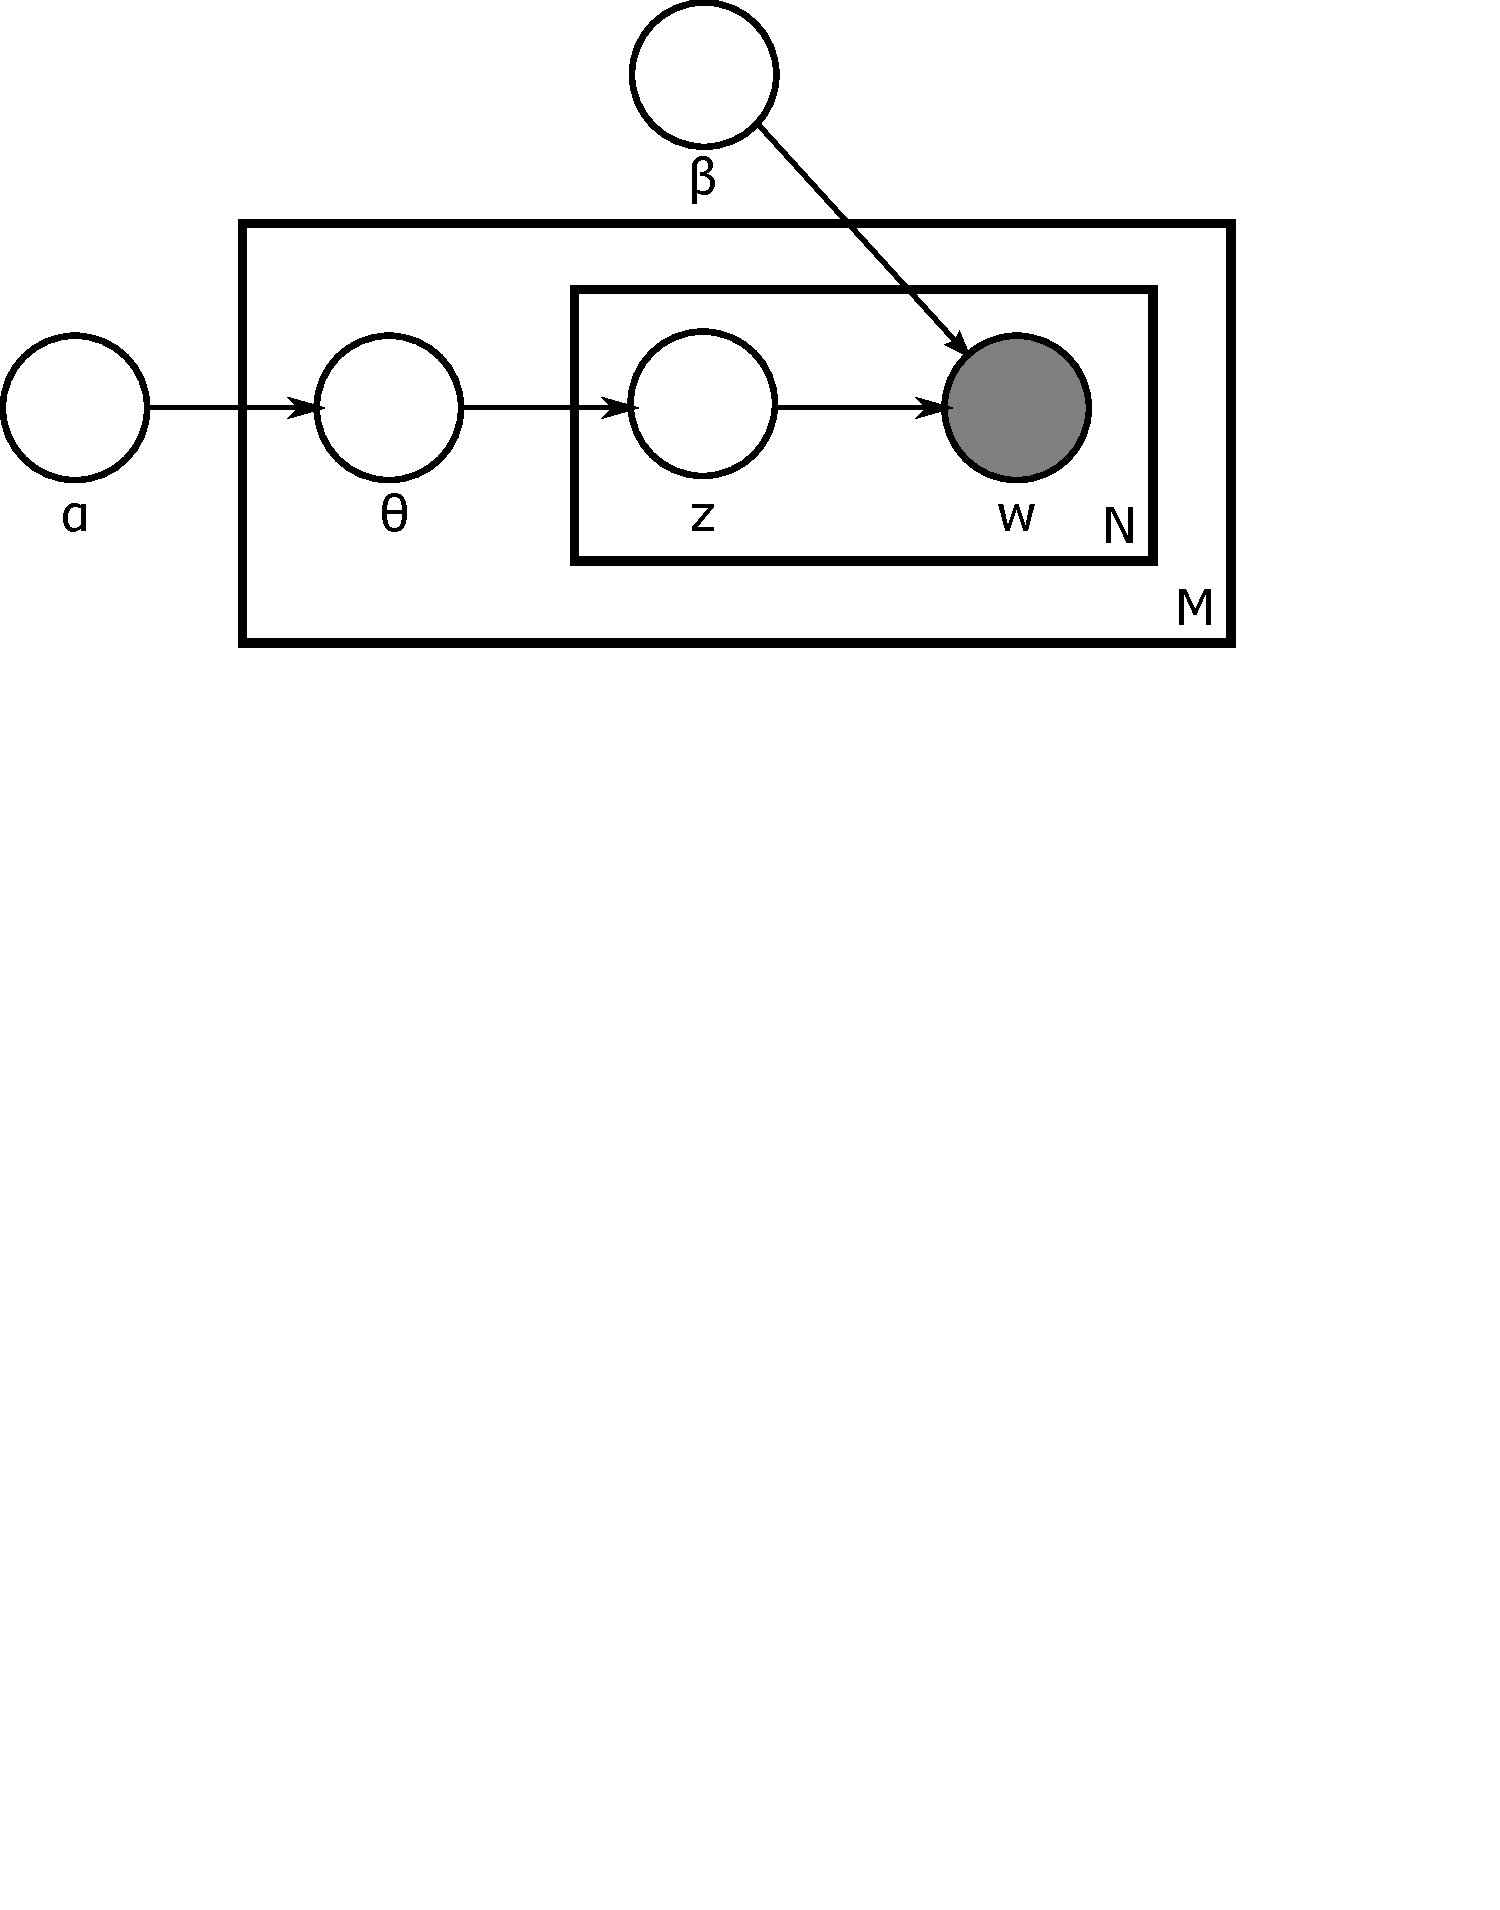
\includegraphics[width=4in]{Latent_Dirichlet_allocation_graphical.pdf}
        \caption{}
      \label{tab:LDA_PlateNotation}
%  \end{center}
\end{figure}

With plate notation, the dependencies among the many variables can be captured concisely. The boxes are “plates” representing replicates. The outer plate represents documents, while the inner plate represents the repeated choice of topics and words within a document. M denotes the number of documents, N the number of words in a document. Thus:

\begin{itemize}
\item{$\alpha$ is the parameter of the Dirichlet prior on the per-document topic distributions;}
\item{$\beta$ is the parameter of the Dirichlet prior on the per-topic word distribution;}
\item{$\theta _{m}$ is the topic distribution for document $m$;}
\item{$\varphi_{k}$ is the word distribution for topic $k$;}
\item{$z_{mn}$ is the topic for the $n$th word in document $m$, and;}
\item{$w_{mn}$ is the specific word.}
\end{itemize}

Plate notation for smoothed LDA::\\
The $w_{ij}$ are the only observable variables, and the other variables are latent variables. Mostly, the basic LDA model will be extended to a smoothed version to gain better results (cite??). The plate notation is shown in Figure~\ref{tab:LDA_PlateNotation}, where $K$ denotes the number of topics considered in the model and:

$\varphi$ is a $\mathbf{K} \times \mathbf{V}$ ($\mathbf{V}$ is the dimension of the vocabulary) Markov matrix (transition matrix), and each row of which denotes the word distribution of a topic.


\subsubsection{Generative Process}
The generative process is as follows. Documents are represented as
random mixtures over latent topics, where each topic is characterized
by a distribution over words. LDA assumes the following generative
process for a corpus $D$ consisting of $M$ documents each of
length $N_{i}$:

\begin{itemize}
\item{1. Choose $\theta _{i}\,   sim \,\mathrm{Dir} (\alpha)$    where $i\in \{1,\dots ,M\}$ and $\mathrm{Dir}(\alpha)$ is the Dirichlet distribution for parameter $\alpha$.}
\item{2. Choose $\varphi _{k}\,\sim \,\mathrm {Dir} (\beta ),$  where $k\in \{1,\dots ,K\}$}.
\item{3. For each of the word positions $i,j$ where 
$j\in \{1,\dots ,N_{i}\} j\in \{1,\dots ,N_{i}\}$, and 
$i\in \{1,\dots ,M\}$:
}
\begin{itemize}
       \item{ (a) Choose a topic $z_{i,j}\,\sim \,\mathrm{Multinomial} (\theta _{i})$.} 
       \item{ (b) Choose a word $w_{i,j}\,\sim \,\mathrm{Multinomial} (\varphi _{z_{i,j}})$.}
         (Note that the Multinomial distribution here refers to the Multinomial with only one trial. It is formally equivalent to the categorical distribution.)
\end{itemize}
\end{itemize}
The lengths $N_{i}$ are treated as independent of all the other data
generating variables ($w$ and $z$). The subscript is often dropped, as
in the plate diagrams shown here.


 


\end{document}


